%%%%%%%% ICML 2025 EXAMPLE LATEX SUBMISSION FILE %%%%%%%%%%%%%%%%%

\documentclass{article}

% Recommended, but optional, packages for figures and better typesetting:
\PassOptionsToPackage{table}{xcolor}
\usepackage{xcolor} 

\usepackage{microtype}
\usepackage{graphicx}
\usepackage{subfigure}
\usepackage{tcolorbox} % Load after xcolor
\usepackage{multirow}
\usepackage{comment}
\usepackage{enumitem}
\usepackage[utf8]{inputenc}
\usepackage[T1]{fontenc}  
\usepackage{lmodern} 
\usepackage{amsmath}
%\usepackage[hyphens]{url}
%\usepackage{hyperref}  
\usepackage[hyphens]{url}
\usepackage{hyperref}
\usepackage[hyphenbreaks]{breakurl}

\usepackage{xurl} % Automatically break URLs
% \usepackage[breaklinks]{hyperref} % Allow hyperlinks to break


\usepackage{tipa}
\usepackage{tikz} % Load after xcolor
\usetikzlibrary{arrows}
\usetikzlibrary{shapes.geometric, positioning, fit}
\usepackage{endnotes}


%\let\footnote=\endnote

% hyperref makes hyperlinks in the resulting PDF.
% If your build breaks (sometimes temporarily if a hyperlink spans a page)
% please comment out the following usepackage line and replace
% \usepackage{icml2025} with \usepackage[nohyperref]{icml2025} above.
\usepackage{hyperref}


% Attempt to make hyperref and algorithmic work together better:
\newcommand{\theHalgorithm}{\arabic{algorithm}}

% Use the following line for the initial blind version submitted for review:
% \usepackage{icml2025}

% If accepted, instead use the following line for the camera-ready submission:
\usepackage[accepted]{icml2025}

% For theorems and such
\usepackage{amsmath}
\usepackage{amssymb}
\usepackage{mathtools}
\usepackage{amsthm}

% if you use cleveref..
\usepackage[capitalize,noabbrev]{cleveref}

%%%%%%%%%%%%%%%%%%%%%%%%%%%%%%%%
% THEOREMS
%%%%%%%%%%%%%%%%%%%%%%%%%%%%%%%%
\theoremstyle{plain}
\newtheorem{theorem}{Theorem}[section]
\newtheorem{proposition}[theorem]{Proposition}
\newtheorem{lemma}[theorem]{Lemma}
\newtheorem{corollary}[theorem]{Corollary}
\theoremstyle{definition}
\newtheorem{definition}[theorem]{Definition}
\newtheorem{assumption}[theorem]{Assumption}
\theoremstyle{remark}
\newtheorem{remark}[theorem]{Remark}

% Todonotes is useful during development; simply uncomment the next line
%    and comment out the line below the next line to turn off comments
%\usepackage[disable,textsize=tiny]{todonotes}
\usepackage[textsize=tiny]{todonotes}


% The \icmltitle you define below is probably too long as a header.
% Therefore, a short form for the running title is supplied here:
\icmltitlerunning{}

\begin{document}

\twocolumn[
\icmltitle{Bridge the Gaps between Machine Unlearning and AI Regulation}

% It is OKAY to include author information, even for blind
% submissions: the style file will automatically remove it for you
% unless you've provided the [accepted] option to the icml2025
% package.

% List of affiliations: The first argument should be a (short)
% identifier you will use later to specify author affiliations
% Academic affiliations should list Department, University, City, Region, Country
% Industry affiliations should list Company, City, Region, Country

% You can specify symbols, otherwise they are numbered in order.
% Ideally, you should not use this facility. Affiliations will be numbered
% in order of appearance and this is the preferred way.
\icmlsetsymbol{equal}{*}

\begin{icmlauthorlist}
\icmlauthor{Bill Marino}{equal,yyy}
\icmlauthor{Meghdad Kurmanji}{equal,yyy}
\icmlauthor{Nicholas D. Lane}{yyy}
% \icmlauthor{Firstname3 Lastname3}{comp}
% \icmlauthor{Firstname4 Lastname4}{sch}
% \icmlauthor{Firstname5 Lastname5}{yyy}
% \icmlauthor{Firstname6 Lastname6}{sch,yyy,comp}
% \icmlauthor{Firstname7 Lastname7}{comp}
%\icmlauthor{}{sch}
% \icmlauthor{Firstname8 Lastname8}{sch}
% \icmlauthor{Firstname8 Lastname8}{yyy,comp}
%\icmlauthor{}{sch}
%\icmlauthor{}{sch}
\end{icmlauthorlist}

\icmlaffiliation{yyy}{Department of Computer Science and Technology, University of Cambridge, Cambridge, UK}
% \icmlaffiliation{comp}{Company Name, Location, Country}
% \icmlaffiliation{sch}{School of ZZZ, Institute of WWW, Location, Country}

\icmlcorrespondingauthor{Bill Marino}{wlm27@cam.ac.uk}
% \icmlcorrespondingauthor{Firstname2 Lastname2}{first2.last2@www.uk}

% You may provide any keywords that you
% find helpful for describing your paper; these are used to populate
% the "keywords" metadata in the PDF but will not be shown in the document
\icmlkeywords{Machine Learning, ICML}

\vskip 0.3in
]

% this must go after the closing bracket ] following \twocolumn[ ...

% This command actually creates the footnote in the first column
% listing the affiliations and the copyright notice.
% The command takes one argument, which is text to display at the start of the footnote.
% The \icmlEqualContribution command is standard text for equal contribution.
% Remove it (just {}) if you do not need this facility.

%\printAffiliationsAndNotice{}  % leave blank if no need to mention equal contribution
\printAffiliationsAndNotice{\icmlEqualContribution} % otherwise use the standard text.

\begin{abstract}
\begin{abstract}  
Test time scaling is currently one of the most active research areas that shows promise after training time scaling has reached its limits.
Deep-thinking (DT) models are a class of recurrent models that can perform easy-to-hard generalization by assigning more compute to harder test samples.
However, due to their inability to determine the complexity of a test sample, DT models have to use a large amount of computation for both easy and hard test samples.
Excessive test time computation is wasteful and can cause the ``overthinking'' problem where more test time computation leads to worse results.
In this paper, we introduce a test time training method for determining the optimal amount of computation needed for each sample during test time.
We also propose Conv-LiGRU, a novel recurrent architecture for efficient and robust visual reasoning. 
Extensive experiments demonstrate that Conv-LiGRU is more stable than DT, effectively mitigates the ``overthinking'' phenomenon, and achieves superior accuracy.
\end{abstract}  
\end{abstract}

\section{Introduction}
\label{introduction}
\section{Introduction}
\label{sec:introduction}
The business processes of organizations are experiencing ever-increasing complexity due to the large amount of data, high number of users, and high-tech devices involved \cite{martin2021pmopportunitieschallenges, beerepoot2023biggestbpmproblems}. This complexity may cause business processes to deviate from normal control flow due to unforeseen and disruptive anomalies \cite{adams2023proceddsriftdetection}. These control-flow anomalies manifest as unknown, skipped, and wrongly-ordered activities in the traces of event logs monitored from the execution of business processes \cite{ko2023adsystematicreview}. For the sake of clarity, let us consider an illustrative example of such anomalies. Figure \ref{FP_ANOMALIES} shows a so-called event log footprint, which captures the control flow relations of four activities of a hypothetical event log. In particular, this footprint captures the control-flow relations between activities \texttt{a}, \texttt{b}, \texttt{c} and \texttt{d}. These are the causal ($\rightarrow$) relation, concurrent ($\parallel$) relation, and other ($\#$) relations such as exclusivity or non-local dependency \cite{aalst2022pmhandbook}. In addition, on the right are six traces, of which five exhibit skipped, wrongly-ordered and unknown control-flow anomalies. For example, $\langle$\texttt{a b d}$\rangle$ has a skipped activity, which is \texttt{c}. Because of this skipped activity, the control-flow relation \texttt{b}$\,\#\,$\texttt{d} is violated, since \texttt{d} directly follows \texttt{b} in the anomalous trace.
\begin{figure}[!t]
\centering
\includegraphics[width=0.9\columnwidth]{images/FP_ANOMALIES.png}
\caption{An example event log footprint with six traces, of which five exhibit control-flow anomalies.}
\label{FP_ANOMALIES}
\end{figure}

\subsection{Control-flow anomaly detection}
Control-flow anomaly detection techniques aim to characterize the normal control flow from event logs and verify whether these deviations occur in new event logs \cite{ko2023adsystematicreview}. To develop control-flow anomaly detection techniques, \revision{process mining} has seen widespread adoption owing to process discovery and \revision{conformance checking}. On the one hand, process discovery is a set of algorithms that encode control-flow relations as a set of model elements and constraints according to a given modeling formalism \cite{aalst2022pmhandbook}; hereafter, we refer to the Petri net, a widespread modeling formalism. On the other hand, \revision{conformance checking} is an explainable set of algorithms that allows linking any deviations with the reference Petri net and providing the fitness measure, namely a measure of how much the Petri net fits the new event log \cite{aalst2022pmhandbook}. Many control-flow anomaly detection techniques based on \revision{conformance checking} (hereafter, \revision{conformance checking}-based techniques) use the fitness measure to determine whether an event log is anomalous \cite{bezerra2009pmad, bezerra2013adlogspais, myers2018icsadpm, pecchia2020applicationfailuresanalysispm}. 

The scientific literature also includes many \revision{conformance checking}-independent techniques for control-flow anomaly detection that combine specific types of trace encodings with machine/deep learning \cite{ko2023adsystematicreview, tavares2023pmtraceencoding}. Whereas these techniques are very effective, their explainability is challenging due to both the type of trace encoding employed and the machine/deep learning model used \cite{rawal2022trustworthyaiadvances,li2023explainablead}. Hence, in the following, we focus on the shortcomings of \revision{conformance checking}-based techniques to investigate whether it is possible to support the development of competitive control-flow anomaly detection techniques while maintaining the explainable nature of \revision{conformance checking}.
\begin{figure}[!t]
\centering
\includegraphics[width=\columnwidth]{images/HIGH_LEVEL_VIEW.png}
\caption{A high-level view of the proposed framework for combining \revision{process mining}-based feature extraction with dimensionality reduction for control-flow anomaly detection.}
\label{HIGH_LEVEL_VIEW}
\end{figure}

\subsection{Shortcomings of \revision{conformance checking}-based techniques}
Unfortunately, the detection effectiveness of \revision{conformance checking}-based techniques is affected by noisy data and low-quality Petri nets, which may be due to human errors in the modeling process or representational bias of process discovery algorithms \cite{bezerra2013adlogspais, pecchia2020applicationfailuresanalysispm, aalst2016pm}. Specifically, on the one hand, noisy data may introduce infrequent and deceptive control-flow relations that may result in inconsistent fitness measures, whereas, on the other hand, checking event logs against a low-quality Petri net could lead to an unreliable distribution of fitness measures. Nonetheless, such Petri nets can still be used as references to obtain insightful information for \revision{process mining}-based feature extraction, supporting the development of competitive and explainable \revision{conformance checking}-based techniques for control-flow anomaly detection despite the problems above. For example, a few works outline that token-based \revision{conformance checking} can be used for \revision{process mining}-based feature extraction to build tabular data and develop effective \revision{conformance checking}-based techniques for control-flow anomaly detection \cite{singh2022lapmsh, debenedictis2023dtadiiot}. However, to the best of our knowledge, the scientific literature lacks a structured proposal for \revision{process mining}-based feature extraction using the state-of-the-art \revision{conformance checking} variant, namely alignment-based \revision{conformance checking}.

\subsection{Contributions}
We propose a novel \revision{process mining}-based feature extraction approach with alignment-based \revision{conformance checking}. This variant aligns the deviating control flow with a reference Petri net; the resulting alignment can be inspected to extract additional statistics such as the number of times a given activity caused mismatches \cite{aalst2022pmhandbook}. We integrate this approach into a flexible and explainable framework for developing techniques for control-flow anomaly detection. The framework combines \revision{process mining}-based feature extraction and dimensionality reduction to handle high-dimensional feature sets, achieve detection effectiveness, and support explainability. Notably, in addition to our proposed \revision{process mining}-based feature extraction approach, the framework allows employing other approaches, enabling a fair comparison of multiple \revision{conformance checking}-based and \revision{conformance checking}-independent techniques for control-flow anomaly detection. Figure \ref{HIGH_LEVEL_VIEW} shows a high-level view of the framework. Business processes are monitored, and event logs obtained from the database of information systems. Subsequently, \revision{process mining}-based feature extraction is applied to these event logs and tabular data input to dimensionality reduction to identify control-flow anomalies. We apply several \revision{conformance checking}-based and \revision{conformance checking}-independent framework techniques to publicly available datasets, simulated data of a case study from railways, and real-world data of a case study from healthcare. We show that the framework techniques implementing our approach outperform the baseline \revision{conformance checking}-based techniques while maintaining the explainable nature of \revision{conformance checking}.

In summary, the contributions of this paper are as follows.
\begin{itemize}
    \item{
        A novel \revision{process mining}-based feature extraction approach to support the development of competitive and explainable \revision{conformance checking}-based techniques for control-flow anomaly detection.
    }
    \item{
        A flexible and explainable framework for developing techniques for control-flow anomaly detection using \revision{process mining}-based feature extraction and dimensionality reduction.
    }
    \item{
        Application to synthetic and real-world datasets of several \revision{conformance checking}-based and \revision{conformance checking}-independent framework techniques, evaluating their detection effectiveness and explainability.
    }
\end{itemize}

The rest of the paper is organized as follows.
\begin{itemize}
    \item Section \ref{sec:related_work} reviews the existing techniques for control-flow anomaly detection, categorizing them into \revision{conformance checking}-based and \revision{conformance checking}-independent techniques.
    \item Section \ref{sec:abccfe} provides the preliminaries of \revision{process mining} to establish the notation used throughout the paper, and delves into the details of the proposed \revision{process mining}-based feature extraction approach with alignment-based \revision{conformance checking}.
    \item Section \ref{sec:framework} describes the framework for developing \revision{conformance checking}-based and \revision{conformance checking}-independent techniques for control-flow anomaly detection that combine \revision{process mining}-based feature extraction and dimensionality reduction.
    \item Section \ref{sec:evaluation} presents the experiments conducted with multiple framework and baseline techniques using data from publicly available datasets and case studies.
    \item Section \ref{sec:conclusions} draws the conclusions and presents future work.
\end{itemize}

\section{Machine Unlearning}
\label{background}
To set the stage for our analysis, we set forth, in this section, we define and provide an overview of MU and its key concepts: 

\subsection{Formal Definition of Unlearning}
Let \( M \) be a model trained on a dataset \( D \) using a training algorithm \( A \). Here, we do not distinguish between \( M \) and its parameters, and write \( M = A(D) \). An \textbf{unlearning query} is typically identified by a set of data points to be forgotten, referred to as the \textbf{forget-set} \( D_f \), and the remaining data points called the \textbf{retain-set}, \( D_r = D \setminus D_f \). The goal of an \textbf{unlearning algorithm} \( U \) is to remove from \( M \) the influence of \( D_f \). The outcome is a new model, called the \textbf{unlearned model}, denoted as \( M_u = U(M; D_f, D_r) \). Depending on the unlearning approach, \( U \) may not have access to \( D_r \) \cite{zhao2024unlearningdifficulty}. In MU research, the notion of "removing influence" has been formalized using definitions from \textbf{differential privacy}. We borrow a version of this definition from \citep{ginart2019makingaiforget} as follows:


\textbf{Definition 2.2.1} Assume that \(U\) and \( A \) are stochastic processes. \(U\) is called an \((\epsilon, \delta)\)-unlearner if the distribution of \( A(D_r) \) and \( U(M; D_f, D_r) \) is \((\epsilon, \delta)\)-close. Specifically, two distributions \( \mu \) and \( \nu \) are \((\epsilon, \delta)\)-close if, for all measurable events \( B \), the following inequalities hold: \(\mu(B) \leq e^\epsilon \nu(B) + \delta\) and \(
\nu(B) \leq e^\epsilon \mu(B) + \delta
\).

This definition provides a natural taxonomy for MU algorithms. When \( \epsilon = \delta = 0 \), \( U \) is termed \textbf{exact unlearning}; otherwise, it is referred to as \textbf{approximate unlearning}.

\subsection{Informal Definitions}
While Def. 2.2.1 provides a rigorous mathematical formulation for MU, researchers often rely on informal interpretations, typically phrased as \texttt{removing [\dots] from $M$}. Deriving informal definitions from Def. 2.2.1 is not always straightforward. A key challenge is that the entity to be removed, may not be clearly identifiable --e.g., in generative models, \texttt{[\dots]} often corresponds to a fact or concept that lacks an explicit representation in either $M$ or $D$.

However, we contend that overly broad definitions of MU introduce unnecessary complexity, potentially hindering clear scientific discourse. In this paper we shall limit unlearning to those techniques in ML that modify the parameter-set of the model (e.g. by deleting and retraining, fine-tuning, or adding/removing some parameters). With this condition, MU still can serve as a tool--among others--for applications such as safeguarding and alignment. At the same time, it leaves methods such as guardrailing (or any "output suppression" as per \cite{cooper2024machineunlearningdoesntthink}) independent of MU, which deserve their own distinct discussion and evaluation in the context of regulations and beyond.

%For instance, recent work \cite{cooper2024machineunlearningdoesntthink} encompasses output safeguarding techniques under the umbrella of unlearning. This expansive definition can potentially complicate the development of scientifically precise and generalizable arguments about unlearning, diluting its conceptual clarity.}



\subsection{Evaluation metrics} 

While Definition 2.2.1 is widely accepted in the MU community, it presents several challenges in practical settings. First, some works question whether this definition is necessary or sufficient to achieve true MU \cite{thudi2022necessityauditing}. Second, in large-scale applications, it is computationally infeasible to directly measure the closeness between the distributions \( A(D_r) \) and \( U(M; D_f, D_r) \). As a result, researchers often resort to alternative proxies to verify MU. These proxies include performance metrics (e.g., classification accuracy \citep{golatkar2020eternal} or generative performance using metrics like ROUGE for large language models \citep{maini2024tofutaskfictitiousunlearning}) and privacy attacks, such as membership inference attacks or backdoor attacks \cite{hayes2024inexactunlearning, triantafillou2024arewemakingprogress}.


\subsection{Unlearning Axes} 
Creating a taxonomy for MU depends on the goal and perspective. Instead of suggesting a new taxonomy, here, we outline two key dimensions that help identifying a MU problem: Model Type, and Forget-Set Definition. 

\textbf{Model Type.} MU is studied in both discriminative and generative models. MU algorithms depend on the training objective and the architectures of these models. For example, \textit{Negative Gradient}, a widely used MU strategy, has different formulations in image classifiers \cite{golatkar2020eternal} versus language models \cite{yao2024muofllms}. Within these two broad categories, one can imaging further subcategories based on data type, evaluation metrics, etc. 

\textbf{Forget-Set Definition.} The forget-set, or the target of MU, can take various forms. It usually is in the following forms: a) the entire data class(es), b) individual data points \cite{kurmanji2023unboundedmachineunlearning}, c) shared features across data points \citep{warnecke2021muoflabelsfeatures}, and d) knowledge (also referred to as concepts or behaviors) that transcends direct connections to the training data \citep{gandikota2024unifiedconceptdelete}.

%\subsubsection{Application}
%MU was originally proposed as a solution for compliance with GDPR's "right to be forgotten" in ML models. Although Article 17 does not explicitly mandate the deletion of data from ML models, research in MU has extended the interpretation of the regulation to encompass such models, often without a comprehensive legal analysis. However, recent work \cite{??}, however, has critically examined MU within the framework of GDPR, concluding that only "retraining from scratch" meets the stringent requirements for compliance. Subsequently, MU has been adapted to address other regulatory and ethical challenges. For instance, it has been employed to remove biases from generative models \cite{omkar}, eliminate backdoors introduced into ML models through poisoned data \cite{?}, delete copyrighted content embedded within model training data \cite{?}, and removing outdated data \cite{?}.

\subsection{Trade-offs and risks}
MU algorithms strive to make a balance between three key objectives: \textbf{Model Utility}, \textbf{Forgetting Quality}, and \textbf{Efficiency}. In certain privacy-centric applications, forgetting can be synonymous with achieving privacy \citep{liu2024breaking}. Hyperparameters and regularizers impact these trade-offs. For example, in MU via \texttt{Fine-tune}, the number of steps and learning rate dictate the balance between forgetting quality and efficiency. Similarly, in \texttt{Gradient Ascent}, the number of steps determines the trade-off between effective MU and preserving model's utility.

Additionally, forgetting may sometimes conflict with privacy due to two phenomena. First, unlearning specific data points can inadvertently expose information about others in the retained set due to the "onion effect" of privacy \citep{carlini2022privacyonioneffectmemorization}. Second, over-forgetting \citep{kurmanji2023unboundedmachineunlearning} a data point may reveal its membership in the original training set—a phenomenon known as the "Streisand Effect" \citep{golatkar2020eternal}. Addressing these challenges requires careful calibration of MU methods to ensure a delicate equilibrium across these competing objectives. These trade-offs are illustrated in \autoref{fig:updated-tradeoffs-diagram}.

Beyond these trade-offs, MU introduces risks associated with \textit{untrusted parties} \citep{li2024pseudounlearning} and \textit{malicious unlearning} \citep{qian2023towardsmaliciousunlearning}. Malicious entities could exploit MU to make fake deletion queries, or introduce computation overheads to the system \citep{marchant2022hardtoforget}.

% \begin{figure}[h!]
%     \centering
%     \resizebox{\columnwidth}{!}{% Resize the entire TikZ picture to fit one column
%         \begin{tikzpicture}[
%             % Define styles for different elements
%             nodeStylePrimary/.style={
%                 draw, 
%                 ellipse, 
%                 text centered, 
%                 minimum height=1.5cm, 
%                 minimum width=3cm, 
%                 font=\bfseries
%             },
%             nodeStyleSecondary/.style={
%                 draw, 
%                 rectangle, 
%                 rounded corners, 
%                 text centered, 
%                 minimum height=1cm, 
%                 minimum width=2cm, 
%                 font=\bfseries
%             },
%             arrowStyleTradeoff/.style={
%                 <->, 
%                 thick, 
%                 solid, 
%                 -latex
%             },
%             arrowStylePrivacy/.style={
%                 <->, 
%                 thick, 
%                 dashed, 
%                 -latex
%             },
%             arrowStyleControl/.style={
%                 ->, 
%                 thick, 
%                 dotted, 
%                 -latex
%             },
%             legendBox/.style={
%                 draw, 
%                 rectangle, 
%                 rounded corners, 
%                 fill=white, 
%                 font=\small,
%                 inner sep=5pt
%             }
%         ]
        
%         % Primary Objectives
%         \node[nodeStylePrimary, fill=blue!30] (Utility) at (0, 0) {Model Utility};
%         \node[nodeStylePrimary, fill=green!30] (Forgetting) at (4, 0) {Forgetting Quality};
%         \node[nodeStylePrimary, fill=orange!30] (Efficiency) at (2, 4) {Efficiency};
        
%         % Privacy as external factor (shifted down slightly)
%         \node[nodeStylePrimary, fill=red!30] (Privacy) at (2, -4) {Privacy};
        
%         % Hyperparameters node (shifted slightly right)
%         \node[nodeStyleSecondary, fill=yellow!30] (Hyperparams) at (6.5, 1.75) {Hyperparameters};
        
%         % Trade-off arrows (solid) with adjusted label positions
%         \draw[arrowStyleTradeoff] (Utility) -- (Forgetting) node[pos=0.6, above] {Balance};
%         \draw[arrowStyleTradeoff] (Forgetting) -- (Efficiency) node[pos=0.6, right] {Trade-off};
%         \draw[arrowStyleTradeoff] (Efficiency) -- (Utility) node[pos=0.4, left] {Trade-off};
        
%         % Privacy relationships (dashed) with shifted labels
%         \draw[arrowStylePrivacy] (Privacy) -- (Forgetting) node[pos=0.4, left] {Conflict};
%         \draw[arrowStylePrivacy] (Privacy) -- (Utility) node[pos=0.6, right] {Impact};
        
%         % Hyperparameters relationships (dotted) with adjusted angles
%         \draw[arrowStyleControl] (Hyperparams) -- (Forgetting) node[pos=0.6, above, sloped] {Adjust};
%         \draw[arrowStyleControl] (Hyperparams) -- (Efficiency) node[pos=0.4, below, sloped] {Tune};
        
%         % Annotations for Privacy Conflicts (shifted slightly outward)
%         \node[draw, diamond, fill=gray!20, minimum size=1cm, above left=0.5cm and 0.5cm of Privacy] (Conflict1) {Info Leak};
%         \node[draw, diamond, fill=gray!20, minimum size=1cm, below left=0.5cm and 0.5cm of Privacy] (Conflict2) {Membership Reveal};
%         \draw[->, dashed] (Privacy) -- (Conflict1);
%         \draw[->, dashed] (Privacy) -- (Conflict2);
        
%         \end{tikzpicture}
%     }
%     \caption{Illustration of the trade-offs in unlearning algorithms among Model Utility, Forgetting Quality, Efficiency, and Privacy. Hyperparameters serve as control elements to navigate these trade-offs. Solid arrows represent direct trade-offs, dashed arrows indicate privacy-related relationships, and dotted arrows denote the influence of hyperparameters.}
%     \label{fig:enhanced-tradeoffs-diagram}
% \end{figure}

\begin{figure}[h!]
    \centering
    \resizebox{0.8\columnwidth}{!}{%
        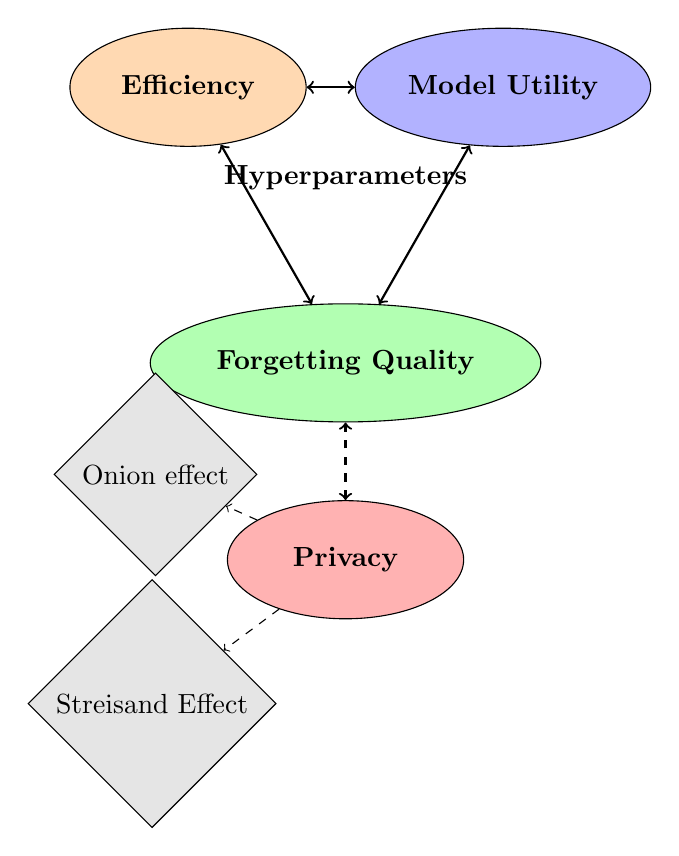
\begin{tikzpicture}[
            % Define styles for different elements
            nodeStylePrimary/.style={
                draw, 
                ellipse, 
                text centered, 
                minimum height=1.5cm, 
                minimum width=3cm, 
                font=\bfseries
            },
            arrowStyleTradeoff/.style={
                <->, 
                thick, 
                solid
            },
            arrowStylePrivacy/.style={
                <->, 
                thick, 
                dashed
            }
        ]
        
        % Repositioned Primary Objectives
        \node[nodeStylePrimary, fill=orange!30] (Efficiency) at (-2, 2) {Efficiency};
        \node[nodeStylePrimary, fill=blue!30] (Utility)    at ( 2, 2) {Model Utility};
        \node[nodeStylePrimary, fill=green!30] (Forgetting) at ( 0,-1.5) {Forgetting Quality};
        
        % Privacy below Forgetting
        \node[nodeStylePrimary, fill=red!30] (Privacy) at (0, -4) {Privacy};
        
        % Trade-off arrows among Efficiency, Utility, and Forgetting (no labels)
        \draw[arrowStyleTradeoff] (Efficiency) -- (Utility);
        \draw[arrowStyleTradeoff] (Efficiency) -- (Forgetting);
        \draw[arrowStyleTradeoff] (Utility)    -- (Forgetting);
        
        % Privacy relationship (dashed) ONLY with Forgetting (no label)
        \draw[arrowStylePrivacy] (Privacy) -- (Forgetting);
        
        % Label inside the triangle
        \node[font=\bfseries] at (0, 0.85) {Hyperparameters};
        
        % (Optional) Privacy conflict annotations (if you still want them)
        \node[draw, diamond, fill=gray!20, minimum size=1cm, above left=-0.1   cm and 0.7cm of Privacy] (Conflict1) {Onion effect};
        \node[draw, diamond, fill=gray!20, minimum size=1cm, below left=0.5cm and 0.6cm of Privacy] (Conflict2) {Streisand Effect};
        \draw[->, dashed] (Privacy) -- (Conflict1);
        \draw[->, dashed] (Privacy) -- (Conflict2);
        
        \end{tikzpicture}
    }
    \caption{\textit{\textbf{Illustration of MU trade-offs.}}}
    \label{fig:updated-tradeoffs-diagram}
\end{figure}



%MU carries several known risks and drawback which are relevant across our analysis. First, data points may be so ``embedded in the model’s implicit knowledge graph'' that it may not be possible to unlearn them without paying a price in model utility \citep{liu_unlearning_2023}. What is more, removing some data points --- e.g., to guard them from confidentiality attacks --- may increase the risk of other data points to the same attacks \citep{carlini2022privacyonioneffectmemorization}.

%\begin{figure}[h!]
\centering
\resizebox{\columnwidth}{!}{ % Resizes the figure to fit the column width
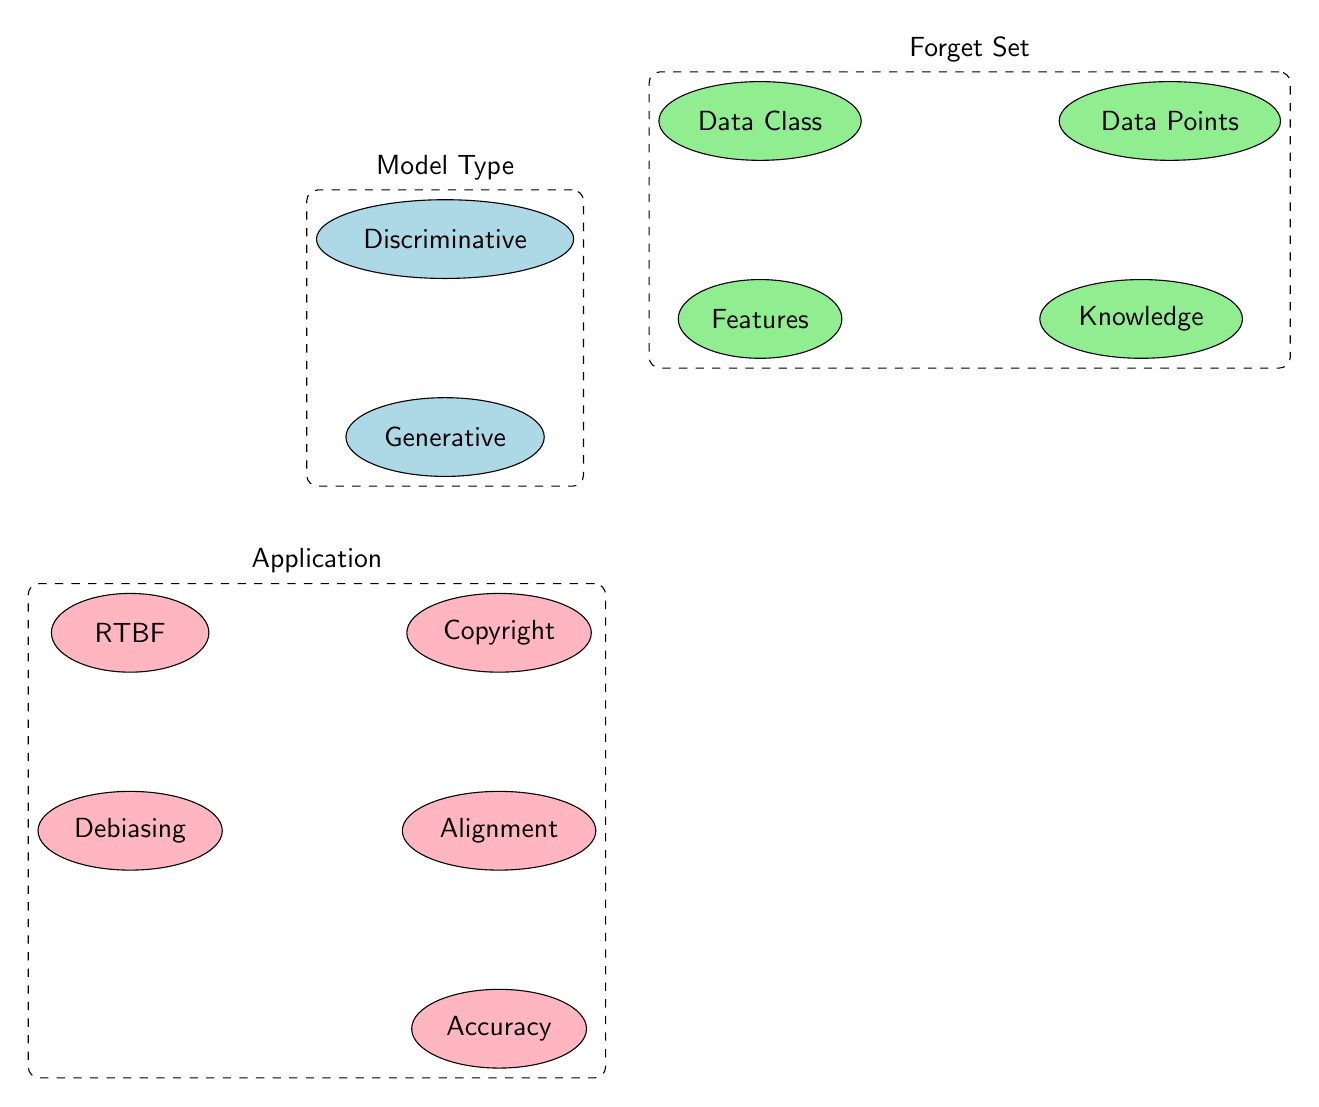
\begin{tikzpicture}[
    every node/.style={font=\sffamily},
    concept/.style={ellipse, draw, text centered, minimum width=2cm, minimum height=1cm},
    group/.style={draw, rounded corners, dashed, inner sep=5mm}
]

% Colors
\definecolor{modelColor}{RGB}{173, 216, 230} % Light Blue
\definecolor{forgetColor}{RGB}{144, 238, 144} % Light Green
\definecolor{applicationColor}{RGB}{255, 182, 193} % Light Pink

% Model Type Group
\node[concept, fill=modelColor] (discriminative) at (0, 0) {Discriminative};
\node[concept, fill=modelColor] (generative) [below=1.5cm of discriminative] {Generative};
\node[draw, rounded corners, dashed, fit={(discriminative) (generative)}, label={above:Model Type}] (modelType) {};

% Forget Set Group
\node[concept, fill=forgetColor] (dataClass) at (4, 1.5) {Data Class};
\node[concept, fill=forgetColor] (dataPoints) [right=2.5cm of dataClass] {Data Points};
\node[concept, fill=forgetColor] (features) [below=1.5cm of dataClass] {Features};
\node[concept, fill=forgetColor] (knowledge) [right=2.5cm of features] {Knowledge};
\node[draw, rounded corners, dashed, fit={(dataClass) (dataPoints) (features) (knowledge)}, label={above:Forget Set}] (forgetSet) {};

% Application Group
\node[concept, fill=applicationColor] (rtbf) at (-4, -5) {RTBF};
\node[concept, fill=applicationColor] (copyright) [right=2.5cm of rtbf] {Copyright};
\node[concept, fill=applicationColor] (debiasing) [below=1.5cm of rtbf] {Debiasing};
\node[concept, fill=applicationColor] (alignment) [below=1.5cm of copyright] {Alignment};
\node[concept, fill=applicationColor] (accuracy) [below=1.5cm of alignment] {Accuracy};
\node[draw, rounded corners, dashed, fit={(rtbf) (copyright) (debiasing) (alignment) (accuracy)}, label={above:Application}] (application) {};

\end{tikzpicture}
} % End of resizebox
\caption{Unlearning dimensions: Model Types, Forget Set, and Applications}
\label{fig:unlearning_dimensions}
\end{figure}


%AI systems developers may be using open-source models without access to the underlying training data \cite{Schneier2024}, meaning that training from scratch is not an option. Even when it is, especially for the models trained on large-scale datasets --- a category that includes many of the most powerful models today -- training from scratch can be "prohibitively costly." \cite{wu2024unlearningconceptsdiffusionmodel,cheng2023gnndeletegeneralstrategyunlearning}.


\section{The EU’s Artificial Intelligence Act}
\label{euaia}
The AIA sets forth harmonized requirements for AI systems and models placed on the market or put into service in the EU \citep[Art. 1]{european_union_ai_act_2024}. These requirements largely target two distinct categories of AI: AI systems and general-purpose AI (``GPAI'') models. Here, we define these two categories and, for each, briefly preview the requirements that, we later argue, MU may assist compliance with.
% Lastly, we outline the relationship between the AIA and GDPR, which also has a bearing on our analysis.

% Its requirements display some particular characteristics and patterns that are worth highlighting because they influence the ways MU could hypothetical be used to aid compliance with the Act.

\subsection{AI Systems}

The AIA broadly defines AI systems to include any ``machine-based system that is designed to operate with varying levels of autonomy and that may exhibit adaptiveness after deployment, and that, for explicit or implicit objectives, infers, from the input it receives, how to generate outputs such as predictions, content, recommendations, or decisions that can influence physical or virtual environments'' \citep[Art. 3.1]{european_union_ai_act_2024}. An example of a system that might meet this criteria is ChatGPT \citep{fernandez-llorca_interdisciplinary_2024}. 

In laying out its rules for these AI systems, the AIA relies on a ``risk-based'' approach \citep{Mahler2022-gc}, by which an AI system's perceived degree of risk determines the exact rules that apply to it. Here, the strictest requirements --- and the ones most relevant to our discussion --- are reserved for those AI systems deemed to be \textit{high-risk} \citep[Art. 6]{european_union_ai_act_2024}. 
% Whether or not an AI system is high-risk is largely based on its intended use \citep{edwards_eu_ai_2022}: specifically, whether the intended use falls into one of the high-risk applications enumerated by the AIA, which include critical infrastructure, education, and more \citep[Art. 6.2; Ann. III]{european_union_ai_act_2024}. 
Such high-risk AI (``HRAI'') systems are subject to a bevy of requirements \citep[Chap. III]{european_union_ai_act_2024}. Among them, the following are the most relevant to our position:\footnote{One set of AIA requirements that we have consciously excluded from our analysis is those around data and data governance for HRAI systems \citep[Art. 10]{european_union_ai_act_2024}. Our interpretation is that these requirements must be met at the dataset level and that no amount of MU on the downstream model will cure violations of these requirements. Ideally, lawmakers or courts will clarify whether our stance is the right one. If it is, then a follow-on question is whether AI system providers who repair Article 10 violations in their data are still obligated to remove the impact of this violative data on models that were trained with it. This question, of course, echoes questions around models trained on datasets that violate GDPR  \citep{JULIUSSEN2023105885, DBLP:conf/sp/BourtouleCCJTZL21, yang2024machinelearningmachineunlearning}. If the answer is in the affirmative, then MU may offer a computational efficient method for doing so --- at least as compared to retraining from scratch. \label{footnote2}}

% HRAI systems must subject their training, evaluation, and test sets (collectively, ``datasets'')  to data governance and management practices appropriate for their intended purpose \citep[Art. 10.2]{european_union_ai_act_2024}. These practices must include measures to detect, prevent and mitigate any ``possible biases that are likely to affect the health and safety of persons, have a negative impact on fundamental rights or lead to discrimination prohibited under Union law'' \citep[Art. 10.2(f-g)]{european_union_ai_act_2024}. These practices must also ``address[]'' any relevant data gaps or shortcomings that prevent compliance with other AIA provisions \citep[Art. 10.2(h)]{european_union_ai_act_2024}. Data governance and management practices aside, datasets must be ``relevant, sufficiently representative, and to the best extent possible, free of errors and complete in view of the intended purpose'' and must display ``appropriate statistical properties'' including as regards the persons or groups of persons in relation to whom the AI system is intended to be used \citep[Art. 10.3]{european_union_ai_act_2024}. The latter, states the AIA's Recitals, necessitates ``the mitigation of possible biases in the data sets'' \citep[Rec. 67]{european_union_ai_act_2024}. Lastly, datasets must ``take into account, to the extent required by the intended purpose, the characteristics or elements that are particular to the specific geographical, contextual, behavioural or functional setting within which the ... AI system is intended to be used'' \citep[Art. 10.4]{european_union_ai_act_2024}.} 


\textbf{Risk management}:
HRAI systems must implement risk management systems that include the identification of known and reasonably foreseeable risks that the system can pose to health and safety or to fundamental rights \citep[Art. 9.2(a)]{european_union_ai_act_2024, kaminski_law_review_2023}. Here, risks to \textit{health and safety}, may include risks to mental and social well-being as well as physical safety. \citep{armstrong_ai_safety_2024, european_commission_ai_qa_2021}. Meanwhile, risks to \textit{fundamental rights} includes risks to any of the rights listed on the EU's Charter of Fundamental Rights \citep{eu_charter_2000}; though, here we only focus on risks to the right most relevant to the topic of MU: the right to non-discrimination, including from biased results \citep{arnold_how_2024}.\footnote{Another fundamental right which some HRAI systems may pose risks to --- risks that must then be managed under \citep[Art. 9]{european_union_ai_act_2024} --- is the right to protection of personal data \citep[Art. 8]{eu_charter_2000}. This includes the right for personal data to ``be processed fairly'' \citep[Art. 8(2)]{eu_charter_2000}, with GDPR subsequently setting the standards for doing so \citep{european_union_gdpr_2016}. Because the application of MU to assist GDRP compliance has been extensively covered by earlier literature \citep{JULIUSSEN2023105885,yang2024machinelearningmachineunlearning} and because our focus is on the \textit{new} use cases for MU brought about by AI regulation, we do not cover it here.}
% As was the case with risks to health and safety, we posit that 
% risks to these two fundamental rights will often stem from problems in the data that MU can, in the downstream model, ostensibly repair. For example, the right to the protection of personal data protects any information relating to an identified or identifiable natural (living) person, including names, dates of birth, photographs, video footage, email addresses, telephone numbers, IP addresses and communications content \citep{edps_dataprotection}. 
Importantly, wherever these risks are identified and can be ``reasonably mitigated or eliminated through the development or design'' of the AI system \citep[Art. 9.3]{european_union_ai_act_2024}, the risk management system must address them with ``appropriate and targeted risk management measures'' \citep[Art. 9.2(d)]{european_union_ai_act_2024}. 
% When choosing these measures, consideration may be given to ``achieving an appropriate balance'' between minimizing the risks and satisfying the AIA's other requirements \citep[Art. 9.4]{european_union_ai_act_2024}. 
These risk management measures must ensure the ``residual risk associated with each hazard, as well as the overall residual risk of the [HRAI] systems is judged to be acceptable'' \citep[Art. 9.5]{european_union_ai_act_2024} and, furthermore, ensure the ``elimination or reduction'' of the identified risks ``as far as technically feasible through adequate design and development''  \citep[Art. 9.5]{european_union_ai_act_2024}.

% \paragraph{\textbf{Data and data governance}:}
% HRAI systems must subject their training, evaluation, and test sets (collectively, ``datasets'')  to data governance and management practices appropriate for their intended purpose \citep[Art. 10.2]{european_union_ai_act_2024}. These practices must include measures to detect, prevent and mitigate any ``possible biases that are likely to affect the health and safety of persons, have a negative impact on fundamental rights or lead to discrimination prohibited under Union law'' \citep[Art. 10.2(f-g)]{european_union_ai_act_2024}. These practices must also ``address[]'' any relevant data gaps or shortcomings that prevent compliance with other AIA provisions \citep[Art. 10.2(h)]{european_union_ai_act_2024}. Data governance and management practices aside, datasets must be ``relevant, sufficiently representative, and to the best extent possible, free of errors and complete in view of the intended purpose'' and must display ``appropriate statistical properties'' including as regards the persons or groups of persons in relation to whom the AI system is intended to be used \citep[Art. 10.3]{european_union_ai_act_2024}. The latter, states the AIA's Recitals, necessitates ``the mitigation of possible biases in the data sets'' \citep[Rec. 67]{european_union_ai_act_2024}. Lastly, datasets must ``take into account, to the extent required by the intended purpose, the characteristics or elements that are particular to the specific geographical, contextual, behavioural or functional setting within which the ... AI system is intended to be used'' \citep[Art. 10.4]{european_union_ai_act_2024}.

\textbf{Accuracy and cybersecurity}: 
HRAI systems must be designed and developed so as to achieve an ``appropriate level'' of accuracy and cybersecurity \citep[Art. 15.1]{european_union_ai_act_2024}. In its Recitals, the AIA stresses that these appropriate levels are a function of the system's intended purpose as well as the SOTA \citep[Rec. 74]{european_union_ai_act_2024}. When it comes to cybersecurity, the AIA specifically requires that HRAI systems be ``resilient against attempts by unauthorised third parties to alter their use, outputs or performance by exploiting system vulnerabilities'' \citep[Art. 15(5)]{european_union_ai_act_2024} and take technical measures to ``prevent, detect, respond to, resolve and control for ... data poisoning'' as well as ``confidentiality attacks'' \citep[Art. 15.5]{european_union_ai_act_2024}.

\subsection{GPAI models}

In contrast to an AI system, a GPAI model is defined as any AI model that is ``trained with a large amount of data using self-supervision at scale, that displays significant generality and is capable of competently performing a wide range of distinct tasks regardless of the way the model is placed on the market and that can be integrated into a variety of downstream systems or applications, except AI models that are used for research, development or prototyping activities before they are placed on the market'' \citep[Art. 3.63]{european_union_ai_act_2024}. Some see this as being synonymous with ``foundation model'' \citep{ada_lovelace_foundation_models_2024}. An example of a GPAI model that might meet this criteria is GPT 3.5, the model powering ChatGPT \citep{fernandez-llorca_interdisciplinary_2024}.

In laying out its requirements for GPAI models, the AIA again uses a risk-based approach, with the strictest requirements reserved for those GPAI models deemed to carry \textit{systemic risk} \citep[Art. 55]{european_union_ai_act_2024}. This is defined as the risk of ``having a significant impact on the [EU] market due to [its] reach, or due to actual or reasonably foreseeable negative effects on public health, safety, public security, fundamental rights, or the society as a whole, that can be propagated at scale across the value chain'' \citep[Art. 2.65; Annex III]{european_union_ai_act_2024}. This status can be established through a number of proxies, including performance on benchmarks and the amount of compute used during training \citep[Art. 51]{european_union_ai_act_2024}. While the AIA itself does not further elaborate on what constitutes systemic risk, the First Draft of the General-Purpose AI Code of Practice, a companion piece to the AIA that breaks it down into more granular technical standards, proposes that it covers risks related to: (1) cyber offense; (2) chemical, biological, radiological, and nuclear (CBRN); (3) loss of control; (4) automated use of models for AI research and development; (5) persuasion and manipulation; and (6) large-scale discrimination \cite{gpai_code_2024}.

Among the AIA's requirements for GPAI models that do display systemic risk --- and those that don't --- the following are the most relevant to our analysis: 

\textbf{Copyright}: 
All GPAI model providers must ``put in place a policy to comply with Union law on copyright and related rights'' \citep[Art. 53.c]{european_union_ai_act_2024}. Among other things, this policy must respect rightsholders' requests, per \citep[Art. 4(3)]{eu_dsg_directive_2019}, to opt out of text and data mining (TDM) on their copyrighted works \citep[Rec. 105, Art. 53.c]{european_union_ai_act_2024}.\footnote{As Recital 105 of the AIA explains, any use of copyright-protected content typically requires the authorization of its rightsholder \citep[Rec. 105]{european_union_ai_act_2024}. While Directive (EU) 2019/790 introduced an exception to this rule for text and data mining, it also granted rightsholders the power to opt out of the exception (unless the text and data mining is done for the purposes of scientific research) \citep[Art. 4]{eu_dsg_directive_2019}. Where the rightsholders opt out, says the AIA, providers of GPAI models must obtain an authorization from rightsholders to carry out text and data mining over their works \citep[Rec. 105]{european_union_ai_act_2024}.}

\textbf{Systemic risk}:
Those GPAI models that display systemic risk are required to ``mitigate'' it \citep[Art. 55(a-b)]{european_union_ai_act_2024}

\textbf{Cybersecurity}: 
GPAI models with systemic risk are additionally required to ``ensure an adequate level of cybersecurity'' \citep[Art. 55(d)]{european_union_ai_act_2024}.



%\begin{table*}[h!]
\centering
\caption{Summary of The European Union’s Artificial Intelligence Act.}
\label{tab:summary_ai_gpai}
\resizebox{\textwidth}{!}{%
\begin{tabular}{|l|l|p{10cm}|}
\hline
\textbf{Category} & \textbf{Key Areas} & \textbf{Details} \\ \hline
\multirow{3}{*}{AI Systems} 
    & Definition & Machine-based systems with autonomy and adaptiveness. Generates outputs like predictions, recommendations, or decisions that impact environments. \\ \cline{2-3}
    & Regulation & Risk-based approach, with stricter rules for high-risk systems. High-risk applications include critical infrastructure, education, and vocational training. \\ \cline{2-3}
    & Key Requirements & 
      - \textbf{Risk Management}: Identify and mitigate risks to health, safety, and fundamental rights. Mitigate risks through appropriate design and development measures. Balance risk minimization with other compliance requirements. \\
      & & - \textbf{Data Governance}: Datasets must be relevant, representative, error-free, and contextually appropriate. Prevent biases and address data gaps or shortcomings. \\
      & & - \textbf{Accuracy and Cybersecurity}: Ensure high accuracy and resilience to threats throughout the system's lifecycle. Protect against vulnerabilities, including data and model poisoning or adversarial attacks. \\ \hline
\multirow{3}{*}{GPAI Models} 
    & Definition & General-purpose AI models trained on large datasets, capable of diverse tasks. Example: GPT-3.5. \\ \cline{2-3}
    & Regulation & Risk-based approach, with stricter rules for models posing systemic risks. Systemic risks include societal impact, public health, and large-scale discrimination. \\ \cline{2-3}
    & Key Requirements & 
      - \textbf{Copyright Compliance}: Adhere to EU copyright laws and respect text and data mining restrictions. \\
      & & - \textbf{Systemic Risk Mitigation}: Address risks like manipulation, discrimination, or public harm. \\
      & & - \textbf{Cybersecurity}: Ensure adequate protection against systemic threats, such as adversarial attacks. \\ \hline
\end{tabular}%
}

\end{table*}


\section{Related Work}
\label{RelatedWork}
\section{RELATED WORK}
\label{sec:relatedwork}
In this section, we describe the previous works related to our proposal, which are divided into two parts. In Section~\ref{sec:relatedwork_exoplanet}, we present a review of approaches based on machine learning techniques for the detection of planetary transit signals. Section~\ref{sec:relatedwork_attention} provides an account of the approaches based on attention mechanisms applied in Astronomy.\par

\subsection{Exoplanet detection}
\label{sec:relatedwork_exoplanet}
Machine learning methods have achieved great performance for the automatic selection of exoplanet transit signals. One of the earliest applications of machine learning is a model named Autovetter \citep{MCcauliff}, which is a random forest (RF) model based on characteristics derived from Kepler pipeline statistics to classify exoplanet and false positive signals. Then, other studies emerged that also used supervised learning. \cite{mislis2016sidra} also used a RF, but unlike the work by \citet{MCcauliff}, they used simulated light curves and a box least square \citep[BLS;][]{kovacs2002box}-based periodogram to search for transiting exoplanets. \citet{thompson2015machine} proposed a k-nearest neighbors model for Kepler data to determine if a given signal has similarity to known transits. Unsupervised learning techniques were also applied, such as self-organizing maps (SOM), proposed \citet{armstrong2016transit}; which implements an architecture to segment similar light curves. In the same way, \citet{armstrong2018automatic} developed a combination of supervised and unsupervised learning, including RF and SOM models. In general, these approaches require a previous phase of feature engineering for each light curve. \par

%DL is a modern data-driven technology that automatically extracts characteristics, and that has been successful in classification problems from a variety of application domains. The architecture relies on several layers of NNs of simple interconnected units and uses layers to build increasingly complex and useful features by means of linear and non-linear transformation. This family of models is capable of generating increasingly high-level representations \citep{lecun2015deep}.

The application of DL for exoplanetary signal detection has evolved rapidly in recent years and has become very popular in planetary science.  \citet{pearson2018} and \citet{zucker2018shallow} developed CNN-based algorithms that learn from synthetic data to search for exoplanets. Perhaps one of the most successful applications of the DL models in transit detection was that of \citet{Shallue_2018}; who, in collaboration with Google, proposed a CNN named AstroNet that recognizes exoplanet signals in real data from Kepler. AstroNet uses the training set of labelled TCEs from the Autovetter planet candidate catalog of Q1–Q17 data release 24 (DR24) of the Kepler mission \citep{catanzarite2015autovetter}. AstroNet analyses the data in two views: a ``global view'', and ``local view'' \citep{Shallue_2018}. \par


% The global view shows the characteristics of the light curve over an orbital period, and a local view shows the moment at occurring the transit in detail

%different = space-based

Based on AstroNet, researchers have modified the original AstroNet model to rank candidates from different surveys, specifically for Kepler and TESS missions. \citet{ansdell2018scientific} developed a CNN trained on Kepler data, and included for the first time the information on the centroids, showing that the model improves performance considerably. Then, \citet{osborn2020rapid} and \citet{yu2019identifying} also included the centroids information, but in addition, \citet{osborn2020rapid} included information of the stellar and transit parameters. Finally, \citet{rao2021nigraha} proposed a pipeline that includes a new ``half-phase'' view of the transit signal. This half-phase view represents a transit view with a different time and phase. The purpose of this view is to recover any possible secondary eclipse (the object hiding behind the disk of the primary star).


%last pipeline applies a procedure after the prediction of the model to obtain new candidates, this process is carried out through a series of steps that include the evaluation with Discovery and Validation of Exoplanets (DAVE) \citet{kostov2019discovery} that was adapted for the TESS telescope.\par
%



\subsection{Attention mechanisms in astronomy}
\label{sec:relatedwork_attention}
Despite the remarkable success of attention mechanisms in sequential data, few papers have exploited their advantages in astronomy. In particular, there are no models based on attention mechanisms for detecting planets. Below we present a summary of the main applications of this modeling approach to astronomy, based on two points of view; performance and interpretability of the model.\par
%Attention mechanisms have not yet been explored in all sub-areas of astronomy. However, recent works show a successful application of the mechanism.
%performance

The application of attention mechanisms has shown improvements in the performance of some regression and classification tasks compared to previous approaches. One of the first implementations of the attention mechanism was to find gravitational lenses proposed by \citet{thuruthipilly2021finding}. They designed 21 self-attention-based encoder models, where each model was trained separately with 18,000 simulated images, demonstrating that the model based on the Transformer has a better performance and uses fewer trainable parameters compared to CNN. A novel application was proposed by \citet{lin2021galaxy} for the morphological classification of galaxies, who used an architecture derived from the Transformer, named Vision Transformer (VIT) \citep{dosovitskiy2020image}. \citet{lin2021galaxy} demonstrated competitive results compared to CNNs. Another application with successful results was proposed by \citet{zerveas2021transformer}; which first proposed a transformer-based framework for learning unsupervised representations of multivariate time series. Their methodology takes advantage of unlabeled data to train an encoder and extract dense vector representations of time series. Subsequently, they evaluate the model for regression and classification tasks, demonstrating better performance than other state-of-the-art supervised methods, even with data sets with limited samples.

%interpretation
Regarding the interpretability of the model, a recent contribution that analyses the attention maps was presented by \citet{bowles20212}, which explored the use of group-equivariant self-attention for radio astronomy classification. Compared to other approaches, this model analysed the attention maps of the predictions and showed that the mechanism extracts the brightest spots and jets of the radio source more clearly. This indicates that attention maps for prediction interpretation could help experts see patterns that the human eye often misses. \par

In the field of variable stars, \citet{allam2021paying} employed the mechanism for classifying multivariate time series in variable stars. And additionally, \citet{allam2021paying} showed that the activation weights are accommodated according to the variation in brightness of the star, achieving a more interpretable model. And finally, related to the TESS telescope, \citet{morvan2022don} proposed a model that removes the noise from the light curves through the distribution of attention weights. \citet{morvan2022don} showed that the use of the attention mechanism is excellent for removing noise and outliers in time series datasets compared with other approaches. In addition, the use of attention maps allowed them to show the representations learned from the model. \par

Recent attention mechanism approaches in astronomy demonstrate comparable results with earlier approaches, such as CNNs. At the same time, they offer interpretability of their results, which allows a post-prediction analysis. \par



\section{MU for AIA compliance: a catalog}
\label{applications}
\definecolor{codeblue}{rgb}{0.25,0.5,0.5}
\lstset{
	backgroundcolor=\color{white},
	basicstyle=\fontsize{7.2pt}{7.2pt}\ttfamily\selectfont,
	breaklines=true,
	keepspaces=true,
	captionpos=b,
	stringstyle=\fontsize{7.2pt}{7.2pt}\color{ApplePrimaryChartRed},
	commentstyle=\fontsize{7.2pt}{7.2pt}\color{ApplePrimaryChartBlue},
	keywordstyle=\fontsize{7.2pt}{7.2pt},
	showstringspaces=false,
}
\begin{lstlisting}[language=Python]
    def find(vector, value):
        """Find locations of value in vector."""
        return np.where(vector == value)[0]

    def remove(vector, value):
        """Find value from vector."""
        return np.delete(vector, find(vector, value))

    def label(vector: np.ndarray, num_classes: int) -> np.ndarray:
        """Return the label in [0, num_classes) for vector."""
        assert len(vector) == 2 * num_classes
        one_hot = vector[num_classes:]
        context = vector[:num_classes]
        i = find(one_hot, 1)
        if context[i] == 0:
            return i
        else:    # remapping
            c = context[i]
            return remove(find(context, c), i)
\end{lstlisting}


\section{Conclusion}
\label{Conclusion}
Despite its many challenges, MU has great potential as a tool for AIA compliance. Because contemporary AI regulations tend to feature recurring principles \citep{doi:10.1080/13510347.2023.2196068, DIAZRODRIGUEZ2023101896}, this likely means that MU has great potential as a tool for compliance with other AI regulations too. To realize this potential, AI researchers should help solve the (sometimes critical) open technical problems logged by this position paper. Among other things, this includes work on identifying forget set data points, on resolving the privacy and performance trade-offs of MU, and on resolving the particular challenges to these use cases that generative model outputs present. While researchers investigate these open problems, lawmakers can support them by explicitly endorsing MU as a compliance tool for AI regulation requirements and, more acutely, resolving some of the particular legal ambiguities we have flagged in this position paper (\ref{footnote2},\ref{footnote7}). Working collaboratively, we can all help unlock MU’s potential to assist compliance with the AI regulation and, by extension, help safeguard the important social values these regulations encode. 

% \section*{Impact Statement}

% In essence, this position paper suggests research directions that will help MU evolve into a better tool for assisting AI regulation compliance. Because these AI regulations tend to protect important ethical and societal values around health and safety, non-discrimination, and more, we believe the impact of this paper, in striving to advance AI regulation compliance through MU, will ultimately be the advancement of those important values as well.

\section*{Acknowledgements}
\textit{Funding}. We wish to acknowledge the Google Academic Research Awards for their support.

% In the unusual situation where you want a paper to appear in the
% references without citing it in the main text, use \nocite

  
\bibliography{example_paper}
\bibliographystyle{icml2025}


%%%%%%%%%%%%%%%%%%%%%%%%%%%%%%%%%%%%%%%%%%%%%%%%%%%%%%%%%%%%%%%%%%%%%%%%%%%%%%%
%%%%%%%%%%%%%%%%%%%%%%%%%%%%%%%%%%%%%%%%%%%%%%%%%%%%%%%%%%%%%%%%%%%%%%%%%%%%%%%
% APPENDIX
%%%%%%%%%%%%%%%%%%%%%%%%%%%%%%%%%%%%%%%%%%%%%%%%%%%%%%%%%%%%%%%%%%%%%%%%%%%%%%%
%%%%%%%%%%%%%%%%%%%%%%%%%%%%%%%%%%%%%%%%%%%%%%%%%%%%%%%%%%%%%%%%%%%%%%%%%%%%%%%
% \newpage
% \appendix
% \onecolumn
% \section{Appendix: End notes.}

% \theendnotes
%%%%%%%%%%%%%%%%%%%%%%%%%%%%%%%%%%%%%%%%%%%%%%%%%%%%%%%%%%%%%%%%%%%%%%%%%%%%%%%
%%%%%%%%%%%%%%%%%%%%%%%%%%%%%%%%%%%%%%%%%%%%%%%%%%%%%%%%%%%%%%%%%%%%%%%%%%%%%%%


\end{document}


% This document was modified from the file originally made available by
% Pat Langley and Andrea Danyluk for ICML-2K. This version was created
% by Iain Murray in 2018, and modified by Alexandre Bouchard in
% 2019 and 2021 and by Csaba Szepesvari, Gang Niu and Sivan Sabato in 2022.
% Modified again in 2023 and 2024 by Sivan Sabato and Jonathan Scarlett.
% Previous contributors include Dan Roy, Lise Getoor and Tobias
% Scheffer, which was slightly modified from the 2010 version by
% Thorsten Joachims & Johannes Fuernkranz, slightly modified from the
% 2009 version by Kiri Wagstaff and Sam Roweis's 2008 version, which is
% slightly modified from Prasad Tadepalli's 2007 version which is a
% lightly changed version of the previous year's version by Andrew
% Moore, which was in turn edited from those of Kristian Kersting and
% Codrina Lauth. Alex Smola contributed to the algorithmic style files.
